\documentclass{article}
\usepackage{tikz,lipsum,lmodern}
\usepackage[english]{babel}
\usepackage[most]{tcolorbox}
\usepackage[paperheight=10.75in,paperwidth=7.25in,margin=1in,heightrounded]{geometry}
\usepackage{graphicx}
\usepackage{blindtext}
\usepackage{ragged2e}
\usepackage{needspace}
\usepackage[space]{grffile}
\usepackage[utf8]{inputenc}
\usepackage[export]{adjustbox}
\usepackage{hyperref}
\usepackage{placeins}
\usepackage{xcolor}
\usepackage{float}

\hypersetup{
    colorlinks,
    citecolor=black,
    filecolor=black,
    linkcolor=black,
    urlcolor=black
}

\usepackage{fancyhdr}
\pagestyle{fancy}
\fancyhf{}
\rhead{\rightmark}
\chead{\thepart}
\lhead{\nouppercase{\leftmark}}
\cfoot{\thepage}
\graphicspath{{"./img/"}}

\title{%
Neural Networks \\
\large Deep Learning}

\author{Silas Hoffmann, inf103088}
\date{\today}


\begin{document}
\maketitle

\vspace{0.5cm}
\tableofcontents
\vspace{1cm}

Notes for the introduction to neural networks presented by \textbf{3blue1brown}. Watch the whole series, click \href{https://www.youtube.com/watch?v=aircAruvnKk}{\color{blue} {here}}. This series describes the strategy to recognize handwritten numbers. To navigate to reference / heading just click on the name.


\clearpage
\listoffigures
\clearpage

\section{But what is a neural network?}

% -------------------------------------------------- 

\subsection{Structural overview}

\FloatBarrier

\begin{figure}[h]
	\centering
	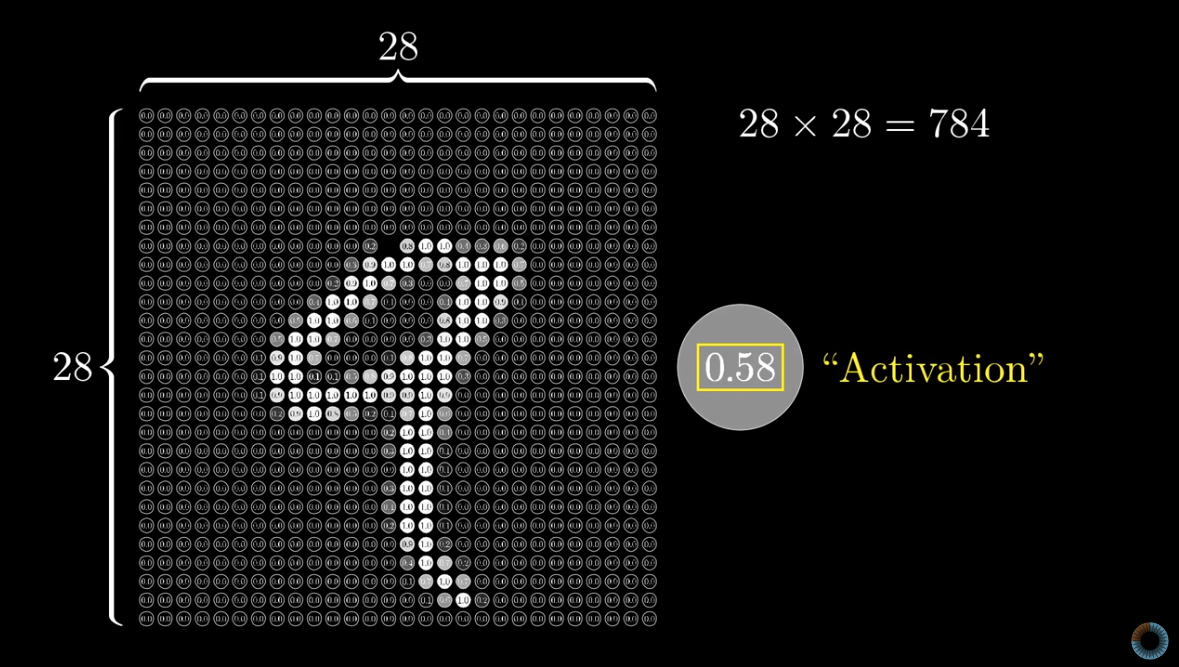
\includegraphics[max width=.9\textwidth]{ai_1}
	\caption{Image interpreted as first layer of neural network}
	\label{ai_1}
\end{figure}

Each pixel from the image is represented by a so called \textit{neuron} (see \ref{ai_1}). These neurons possess a value called \textbf{Activiation} which contains a float between 0 and 1. This value specifies the brightness of this the particular pixel. This activation value also can be interpreted as how \textit{lit up} this particular neuron actually is, 1 meaning 100 \% in this context.

\begin{figure}[b!]
	\centering
	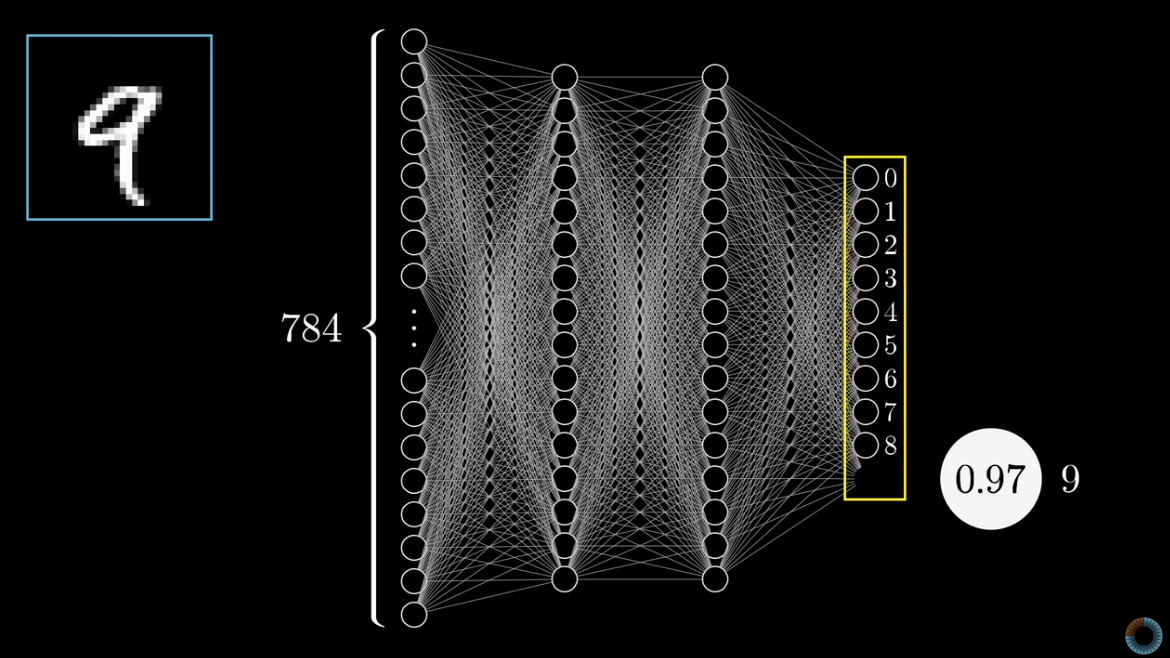
\includegraphics[max width=.9\textwidth]{ai_2}
	\caption{Resulting top layer}
	\label{ai_2}
\end{figure}

As each number is analyzed the top layer gives its prediction to a given input via Activation of the ten most right nodes (see \ref{ai_2}). The one with the highest activation states what the system thinks the correct number might be. The layers between the top and the bottom layer are called \textbf{hidden layers}. 

\begin{figure}[h]
	\centering
	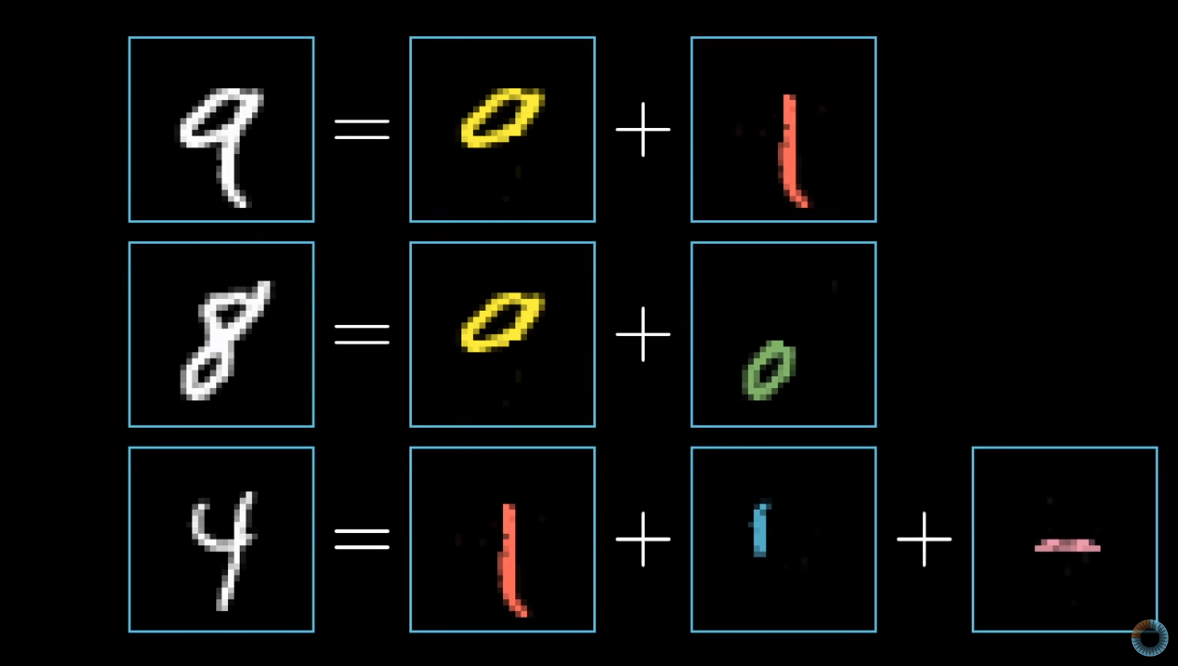
\includegraphics[max width=.9\textwidth]{ai_3}
	\caption{Image interpreted as first layer of neural network}
	\label{ai_3}
\end{figure}

The number of layers is not fixed and can be set to any number appropriate to the problem the system should solve. In this example it is useful to two hidden layers because of how the system works. A handwritten digit can be subdivided into different components (see img. \ref{ai_3}). E.g. the number 9 can be divided into a top loop and a bottom line. These different steps will be analyzed by the various layers from the network. Maybe some digits share specific components and those nodes can be \textit{reused} (see img. \ref{ai_4}). The idea is that any digit with a \textit{loopy} pattern towards the top sends of the specified neuron. This information is then used to fire up neurons in the next layer based on the idea that at least some kind of pattern already fits the input data.

\begin{figure}[h]
	\centering
	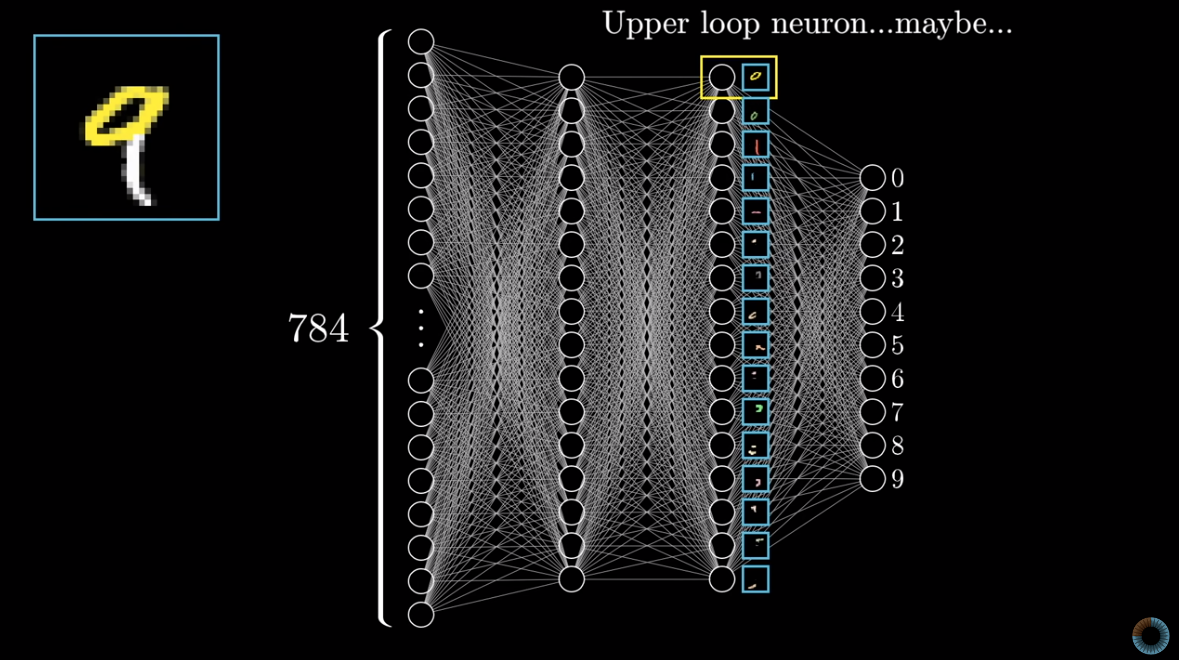
\includegraphics[max width=.9\textwidth]{ai_4}
	\caption{Recognizing more complex patterns via abstraction}
	\label{ai_4}
\end{figure}

But to be capable of recognizing such a complex patterns as a loop, the system has to recognize all the various subcomponents of a loop. Those mainly consist out of small edges which in total form a loop from a wider perspective. This may be the task of the second layer while the third layer is responsible for recognizing those more complex parts (see img. \ref{ai_6}). 

Again, the number of layers is totally arbitrary. It might even be usefull to divide those smaller lines from layer 2 into smaller components, then there might be another layer. Or maybe the second layer is redundant altogether because the system can recognize those complex pattern directly. It always depends on the problem that the network should solve to decide how many layers are actually usefull.

\begin{figure}[h]
	\centering
	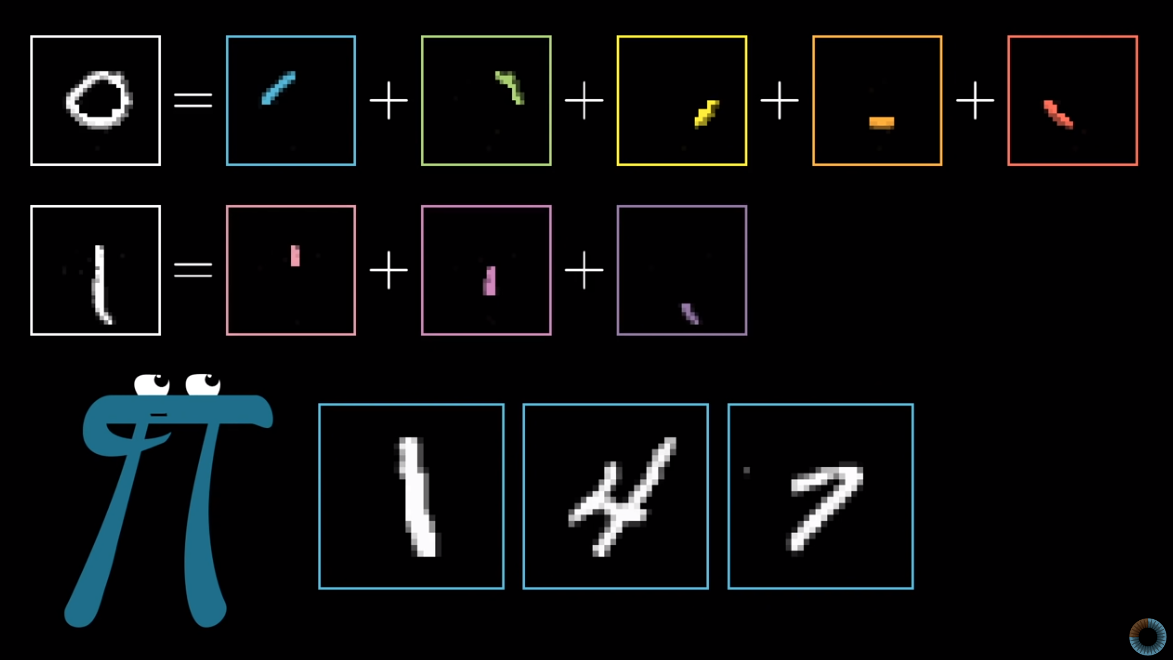
\includegraphics[max width=.9\textwidth]{ai_5}
	\caption{Examples of simple shapes forming complex digits}
	\label{ai_5}
\end{figure}

In a nutshell the different layers in a neural network each describe a certain level of complexity. Those lower levels represent simpler coherence than the ones on top of those. In the next picture you can see the which neurons on each layer may fire when confronted with a sample of a handwritten nine.

\begin{figure}[h]
	\centering
	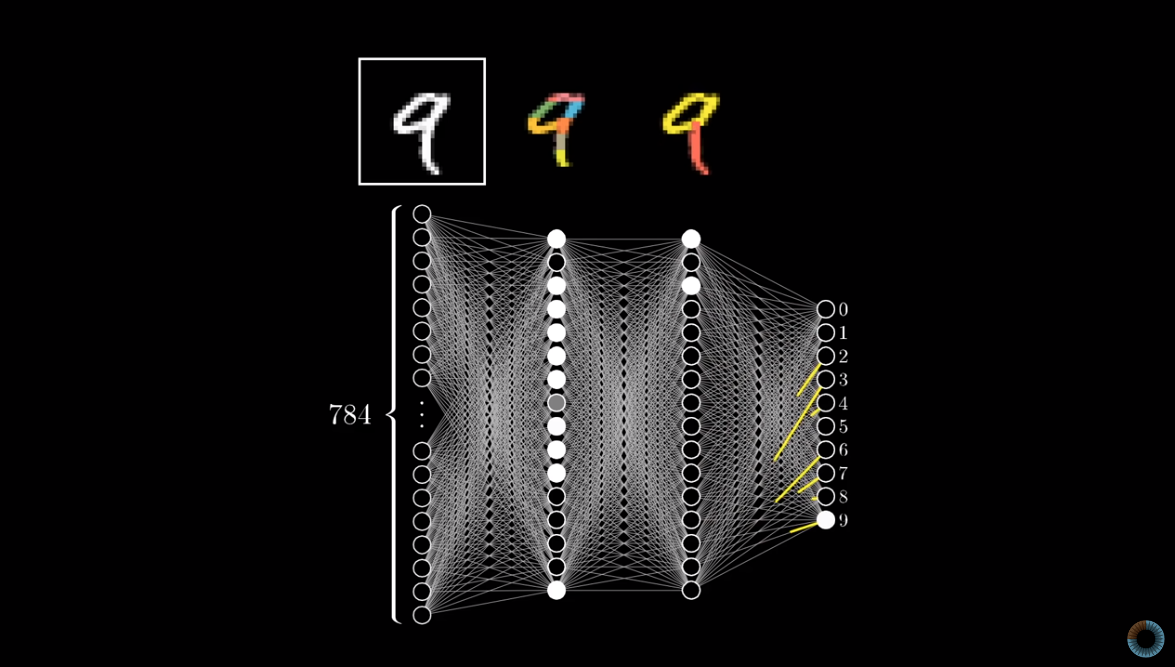
\includegraphics[max width=.9\textwidth]{ai_6}
	\caption{Top to bottom overview}
	\label{ai_6}
\end{figure}

% -------------------------------------------------- 

\subsection{Regognizing patterns}
The main purpose of the given example network is to detect edges of the given digits and from these edges determine patterns which in turn result in a identified digit. But this principle of detecting details and forming a bigger picture is also relevant in other fields e.g. autonomous cars or speeach regognition where a given audio samples consists out of waves which form voices which form words etc. 

To show how it actually works to detect one of those minor details to from the simples \textit{hidden layer} the tutor shows how to recognize a single line in a specific part of the picture (see img. \ref{ai_7}).

\begin{figure}[h]
	\centering
	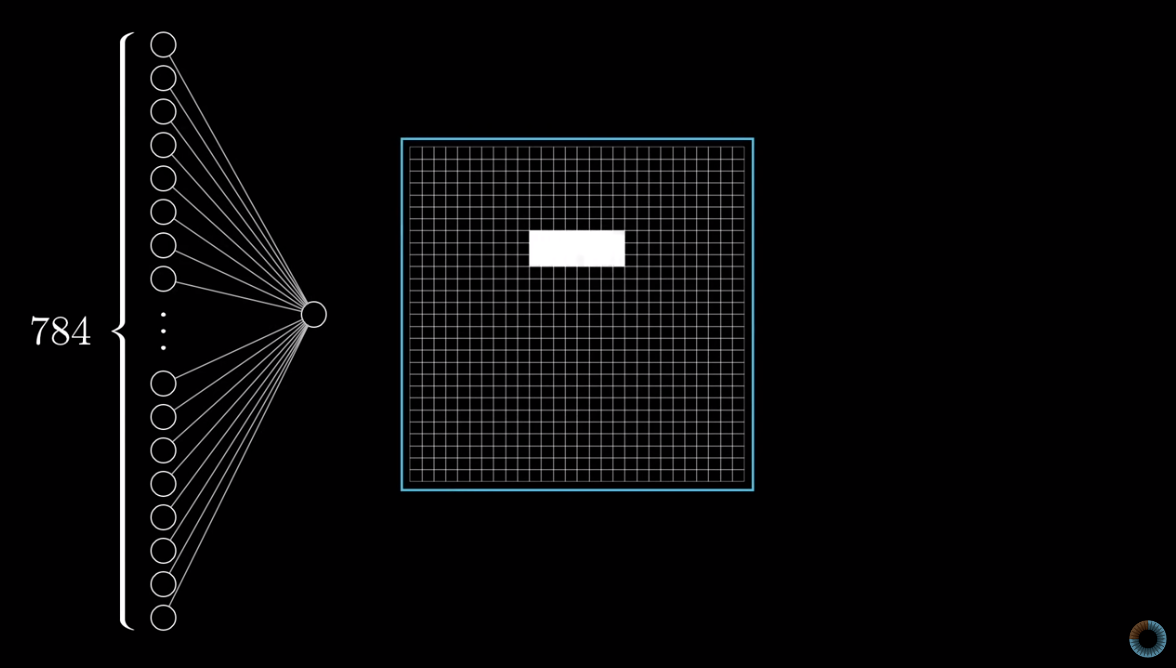
\includegraphics[max width=.9\textwidth]{ai_7}
	\caption{Bounding box for detecting specific line}
	\label{ai_7}
\end{figure}

\begin{figure}[h!]
	\centering
	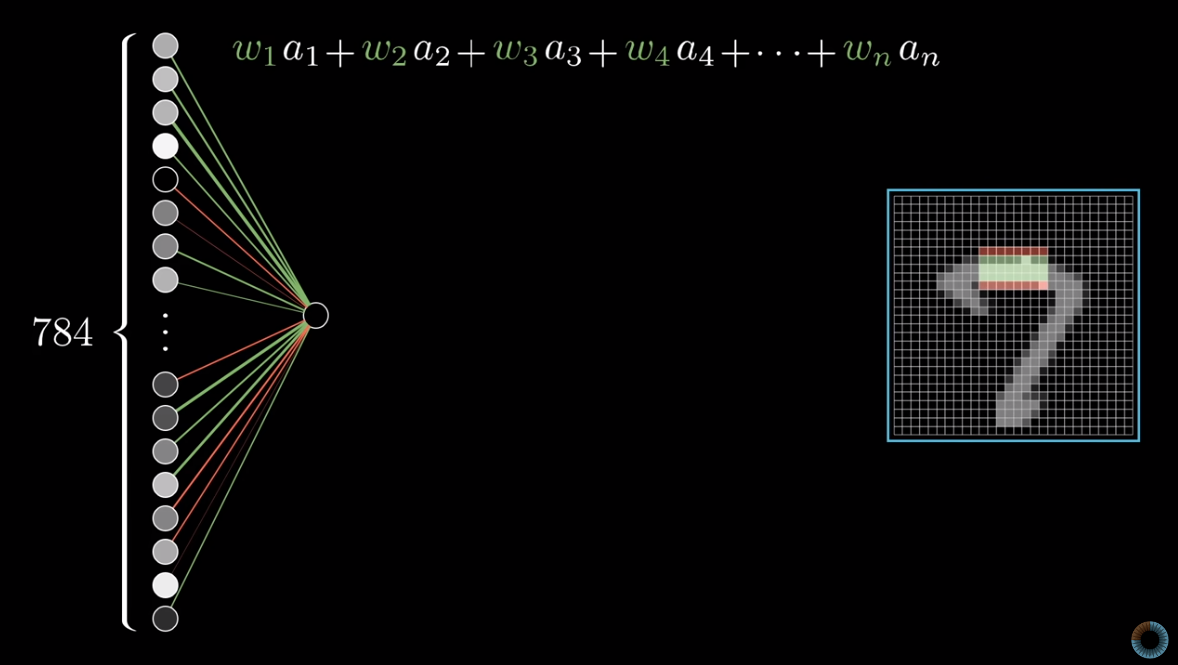
\includegraphics[max width=.9\textwidth]{ai_8}
	\caption{Colored weights for specifying outlines}
	\label{ai_8}
\end{figure}

In the example we try to detect the middle part of the digit seven (see img. \ref{ai_8}). To check whether or not the given pixels have a line in the specified part of the image we assign a so called \textbf{weight} to each of the connections of nodes on the first layer (direct image input) to the node responsible for recognizing the depicted part of the image as a line. To do so each connection outside of the bounding box gets assigned a value of zero and the relevant nodes get a value greater zero. Now each weight will be multiplied with the corresponding node value \textit{(brightness of the node)} and all those values will be added. Whenever there is actually a line in the specified box the sum of the values will be higher than if there wasn't a line. To make it state that we actually expect a line which does not touch the upper and lower bound of the box we can also create negative bounds for the outer pixels which in turn extravagates the result even more. 

E.g. a black line crosses the otherwise completely blank / white canvas. Then the nodes which are expected to be white multiply by a quite big factor with the small values and the outer pixels touch the bound of the box. This will result in some pretty huge negative numbers because the weight are negative in those places. On the other hand, if you put a perfect line that is not touching the bounds in the box then the sum of all products with the weights will be much larger and the neuron will fire a value much \textit{\textbf{brighter}}.

\begin{figure}[h]
	\centering
	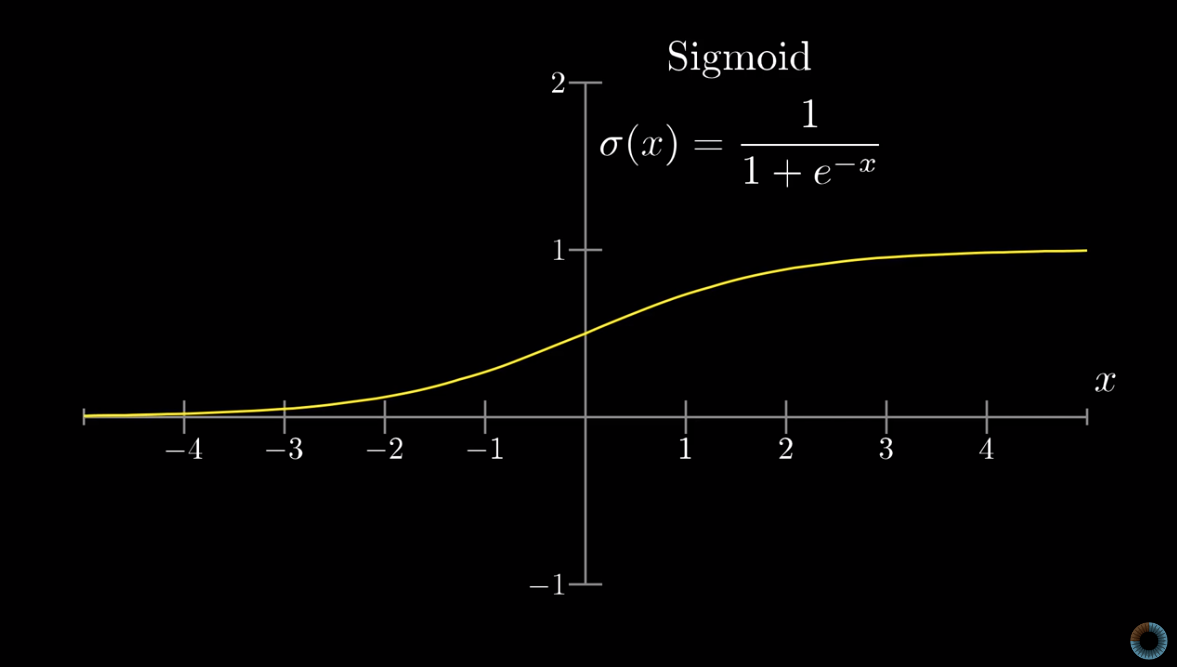
\includegraphics[max width=.9\textwidth]{ai_9}
	\caption{Sigmoid function}
	\label{ai_9}
\end{figure}

Since the calculated sum of the product with the weights may very well be much larger than 1 or smaller than 0, the sum will be squished into the the interval 0 to 1 via some kind of function. Often a function called the \textbf{sigmoid function} is used which creates a value near zero for negative values and a value near 1 for high values (see img. \ref{ai_9}). It is important to limit the output to this interval because it will serve as the \textbf{activision} of the node when the node is used in the next step / layer of the network. 

A very important summary: \textit{The activation of a neuron is basically a measure of how positive the relevant weighted sum is.}


\begin{figure}[h]
	\centering
	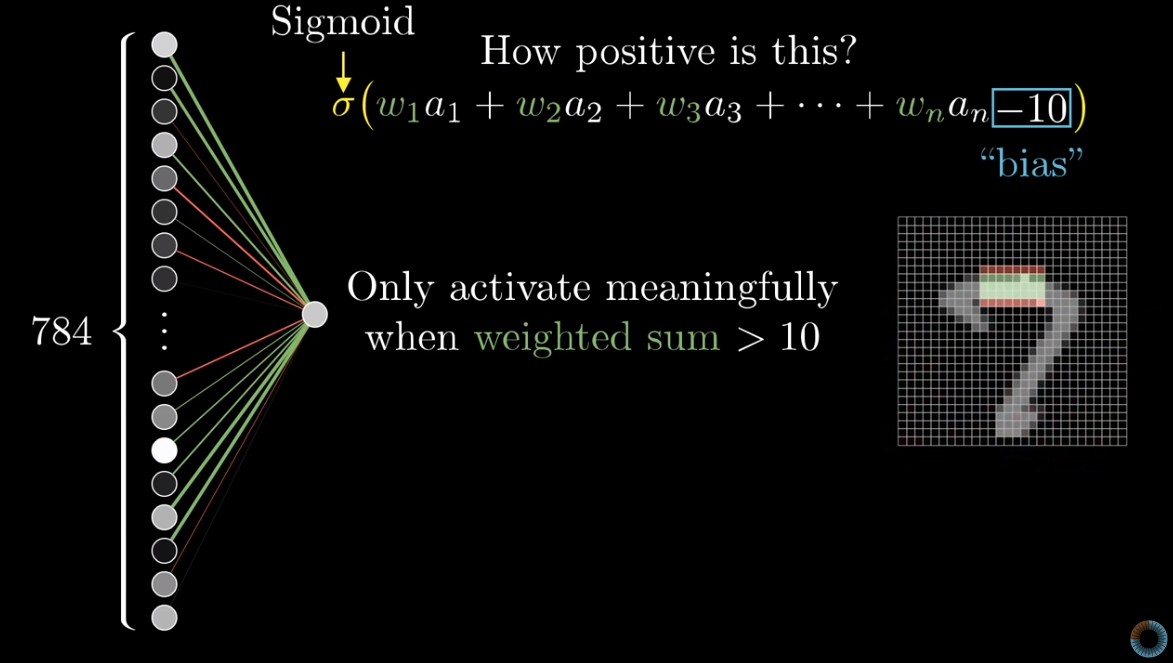
\includegraphics[max width=.9\textwidth]{ai_10}
	\caption{Activation displayed with bias and sigmoid function}
	\label{ai_10}
\end{figure}

Another important tool is the so called \textbf{bias} which acts a sort of lower bound for the activation of the neuron. Say you want the neuron to only detect very thick and bright lines. Then you need this bias to say something like \textit{only light up when weighted sum is greater than 10} (see img. \ref{ai_10}). This can be achived by subtracting the bias inside the sigmoid function.


% -------------------------------------------------- 

\subsection{Notation - Learning process}

\begin{figure}[!htbp]
	\centering
	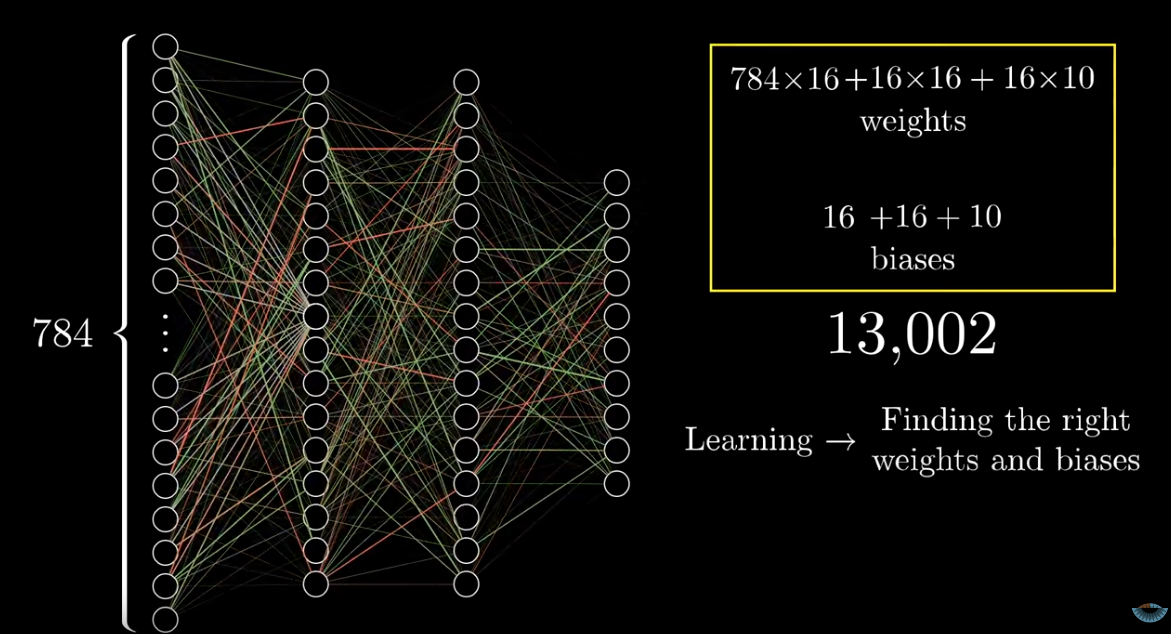
\includegraphics[max width=.9\textwidth]{ai_11}
	\caption{Systemwide number of weights and biases}
	\label{ai_11}
\end{figure}

The \textit{learning process} generally describes the algorithm to set all those weights and biases needed for each and every node in the network. Since the given example network has 784 base input nodes, two hidden layers with 16 nodes each and a 10 node output layer, the whole system all in all has 13 002 values to set (see img. \ref{ai_11}).

\begin{figure}[!htbp]
	\centering
	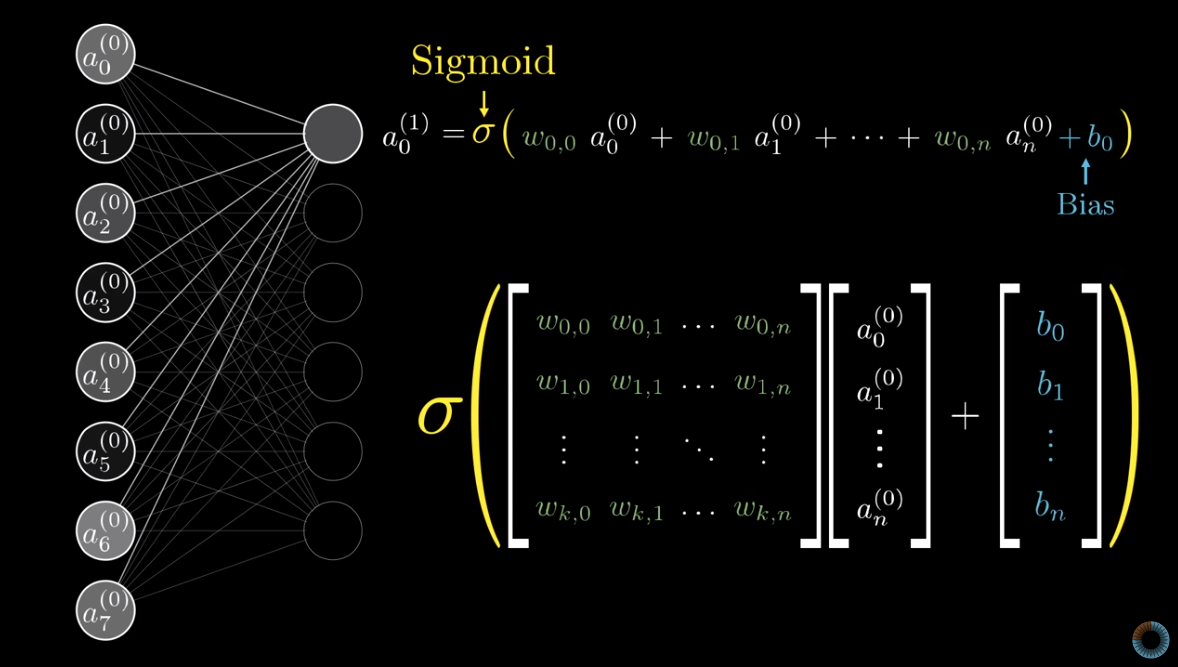
\includegraphics[max width=.9\textwidth]{ai_12}
	\caption{vector notation}
	\label{ai_12}
\end{figure}

To write the value / activation for each node in a more compact way than seen in \ref{ai_10} the vectore notation is being used quite often (see img. \ref{ai_11}). The structure is as follows: First comes the weight matrix. In each row the matrix holds the weight for the connection between a given neuron on the current layer with one particular neuron on the next layer. E.g. the first row holds the information displayed in the picture (see img. \ref{ai_11}). The matrix vector multiplication actually conveys the same information as the stated sum above. The resulting vector represents the activation of the nodes on the next layers. Afterwards a vector containing the bias for each node is being added to the product. To normalize the resulting activations will be transformed with the formally discussed \textbf{sigmoid} function by wrapping this function around everything.




% -------------------------------------------------- 

\section{Gradient descent, how neural networks learn}

The basic idea is that you feed the network with testdata which form the previously discussed connections. During the learning phase the networks gets feedback on how it is performing and how it can improve. Once it is fairly accurate it is expected to be able to recognize pattern outside of the given testdata. To start all this the network gets assigned random numbers in all the weights and biases.

% -------------------------------------------------- 

\subsection{Cost function}

\begin{figure}[!htbp]
	\centering
	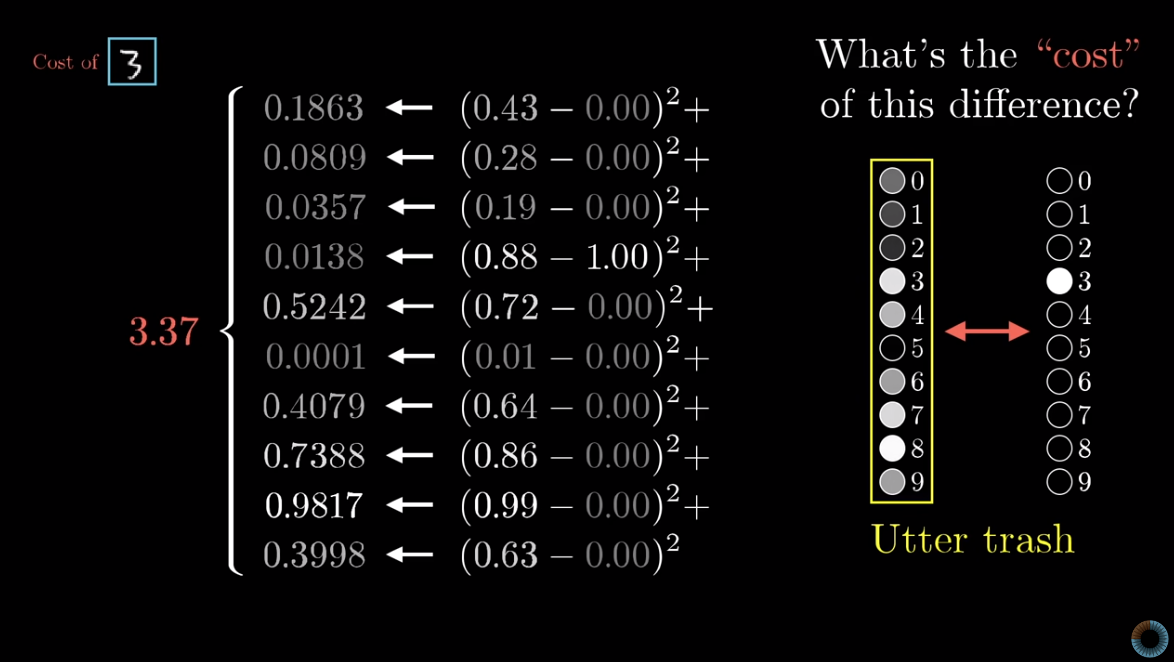
\includegraphics[max width=.9\textwidth]{ai_13}
	\caption{Cost function for one input}
	\label{ai_13}
\end{figure}

To give the network a feedback we need to define a cost function. This function takes an input and checks if the output of the network corresponds with the expected output stated in the testcase. To do so the function calculates the square of difference between the expected and the actual output and adds all those up for all the nodes. E.g. see \ref{ai_13}. The network is not sure which digit it may be and besides the digit one suggest multiple other output digits. In a perfect world all other neurons should have an activation of zero while the neuron with the digit one has an activation of also one. \textit{The \textbf{cost} of the actual output is high while the cost of the optimal output is low.} The \textbf{cost} of the whole network is defined by the average of those costs over all the training data.


To train the network you have to know the minimum of this cost function. Take the following example for minimizing a function taking on input value and generating one output. 

\begin{figure}[!htbp]
	\centering
	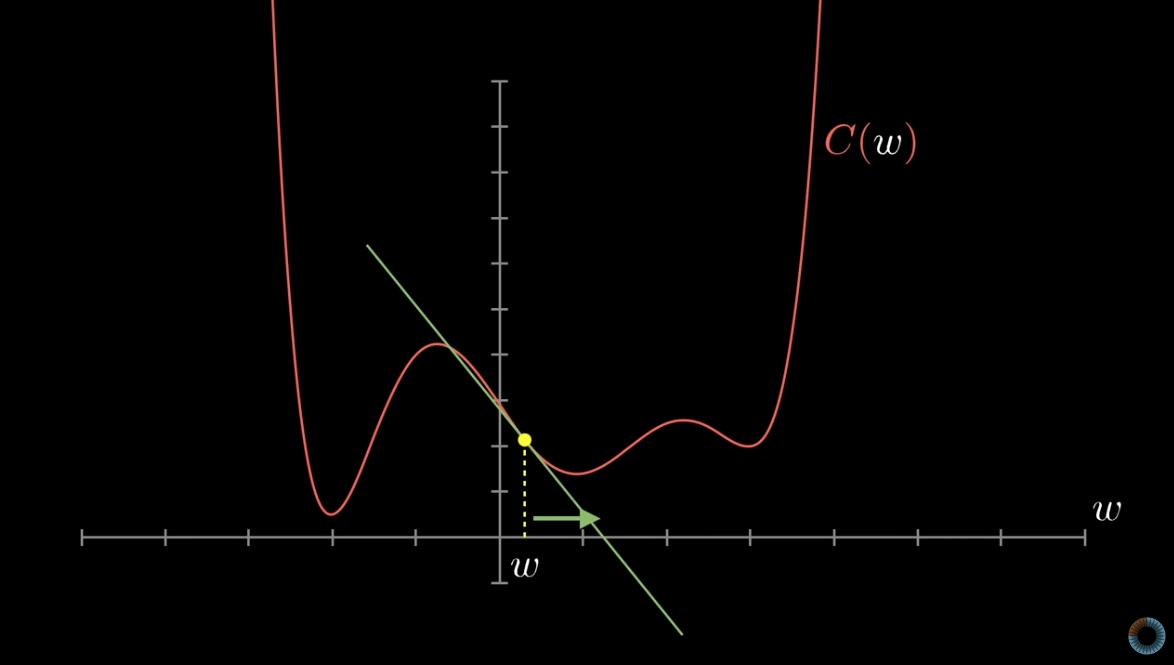
\includegraphics[max width=.9\textwidth]{ai_14}
	\caption{Fining minimum 2d}
	\label{ai_14}
\end{figure}

To generate the next minimum to a given point we take the slope of the function at this point and go to the negative side of the tangent. It is important to mention that the step size for the next point is proporitional to the slope itself. This way we prevent the point from overgoing the minimum. 

But it isn't enough to just take one point and run it with the explained algorithm, there need to be multiple points on the curve to determine the other minimums. Taking this approach we can find more minima and from those findings can determine the best / smallest one. Although we find more minima than before there is not guarantee for finding \textbf{all} minima.

\begin{figure}[!htbp]
	\centering
	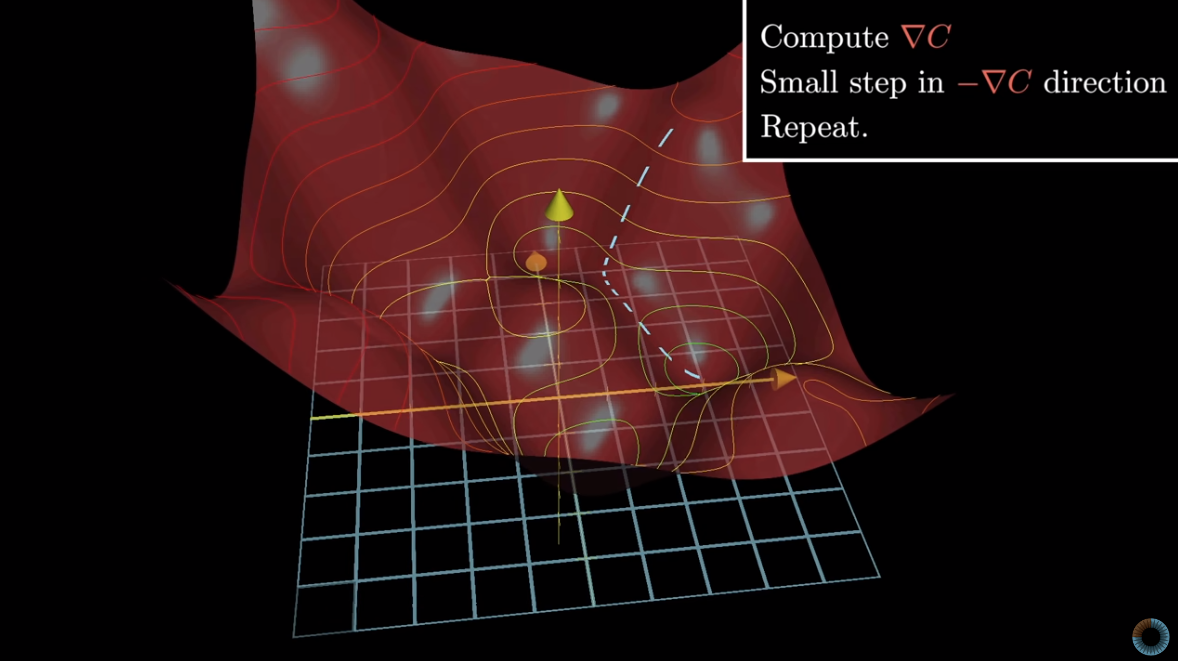
\includegraphics[max width=.9\textwidth]{ai_16}
	\caption{Finding minimum 3d}
	\label{ai_16}
\end{figure}

Now consider a function taking in 2 input values and generating one output value (see img. \ref{ai_14}). We can display this function as a surface on the xy plane in the 3d space. Now the challenge is to find the best minimum here. Again looking at the previous example we need to spread out points over the function where we want to take a look at the direction of the next minimum. To do so we need to take a look at the gradient vector. Inverting this we get a vector point pointing \textit{downhill} to the next minimum (see img. \ref{ai_16}). 

%To put in in perspective with the cost function we need to imagine the 
This principle can be applied to the given cost function of the network. To do so the cost function needs to be interpreted as a function taking all the weights in as parameters and generates a single output values. It is the same as the last example with the 3d space. When interpreting the cost function as some kind of x dimensional surface we need to find the direction for the minimum. As explained this can be done by taking the negative Gradient of the current value. 

\begin{figure}[!htbp]
	\centering
	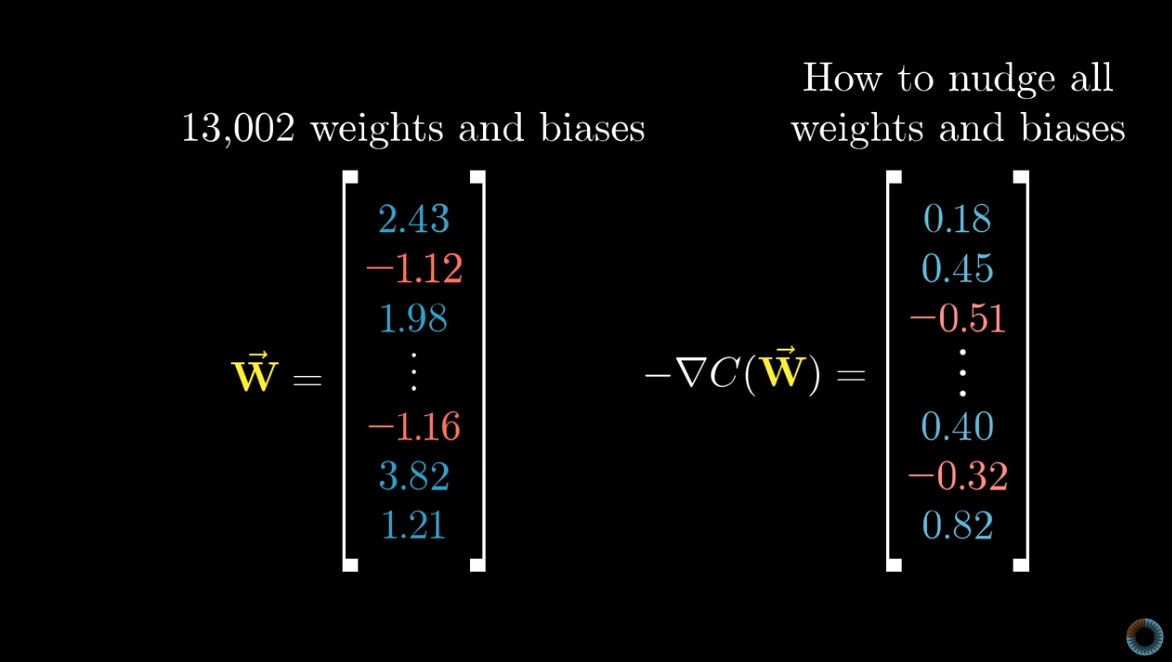
\includegraphics[max width=.9\textwidth]{ai_17}
	\caption{Vector notatio with the negative gradient}
	\label{ai_17}
\end{figure}

To write it in a compacter way we define a vector with all of the networks weights in one column. The cost function takes this vector as an input. We then define the negative Gradient of the cost function and the output can in turn be written as a vector again. In a more colloquial manner: \textit{The output of the negative gradient states the direction of which the Ball rolling downhill needs to take to find the minimum.}

When minimizing the cost function this way we don't minimize the function for one specific training example but for all possible training data samples. The algorithm for computing this gradient efficiently which is effectifly the part of how a neural network learns is called \textbf{backpropagation} (which has its own chapter). 

\begin{figure}[!htbp]
	\centering
	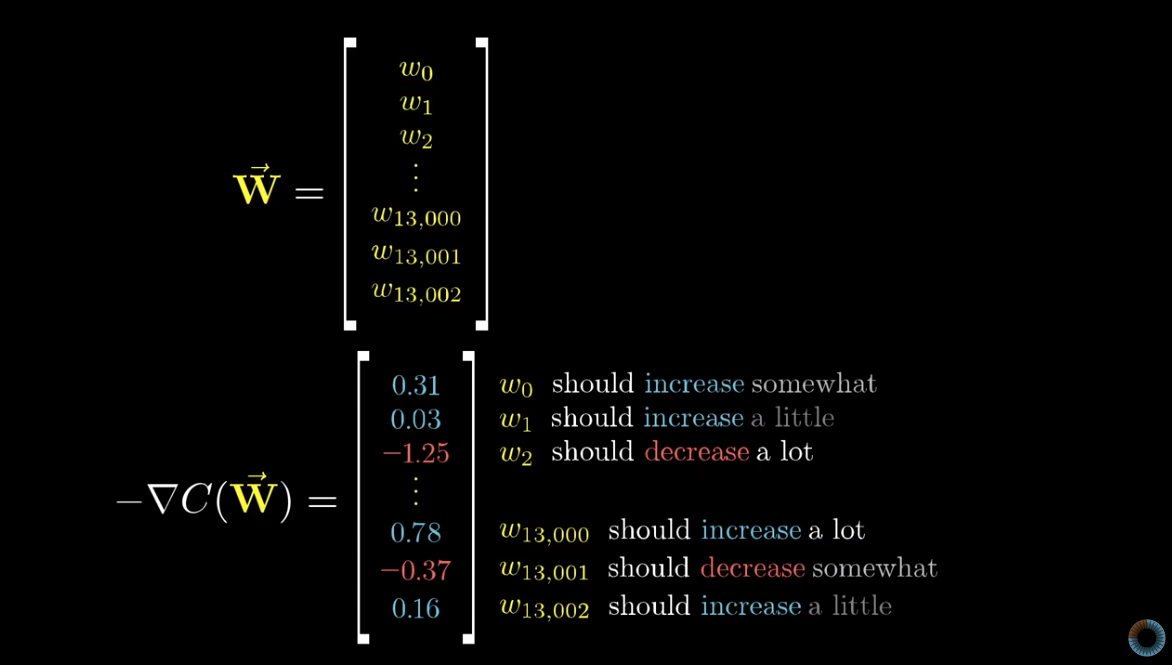
\includegraphics[max width=.9\textwidth]{ai_18}
	\caption{Finding minimum 3d}
	\label{ai_18}
\end{figure}

A way to interpret the given gradient vector is to associate each component value as an indicator for its importance on the overall cost function (see img. \ref{ai_18}). Meaning tweaking a weight with a higher value has more influence on minimizing the cost function than a value with a low value.



% -------------------------------------------------- 

\section{What is backpropagation really doing?}

Backpropagation is a way to compute the gradient to \textit{tell} the neural network what weights need to be changed. 

\subsection{Intiutive walkthrough}

\begin{figure}[!htbp]
	\centering
	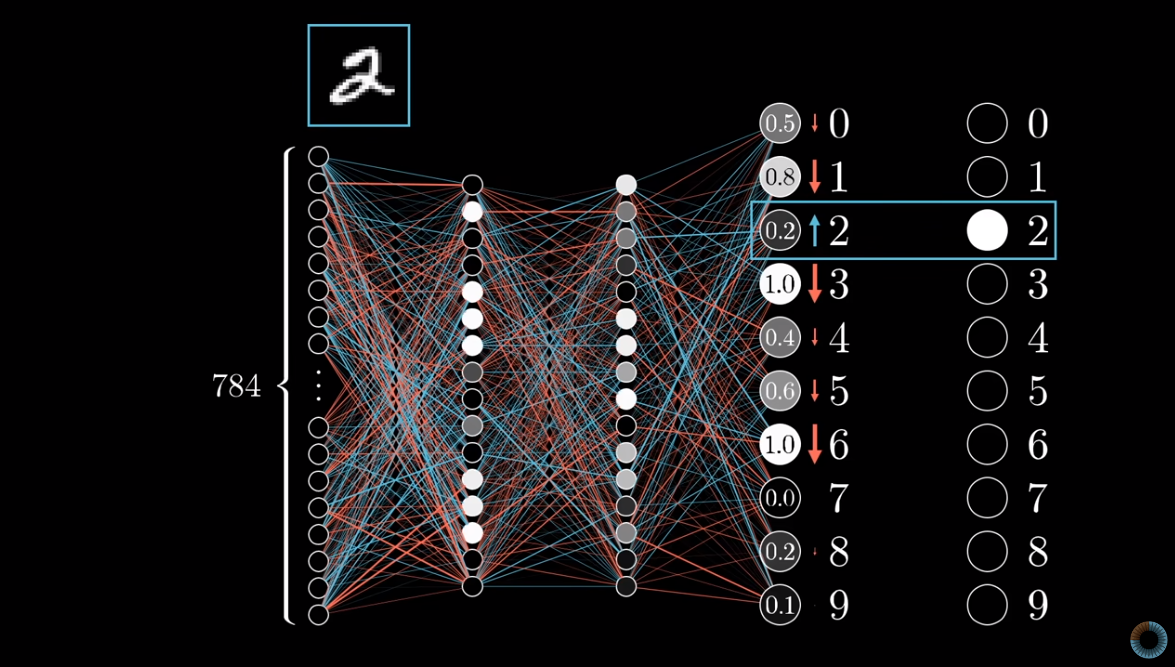
\includegraphics[max width=.9\textwidth]{ai_19}
	\caption{Desired changes to previous layer}
	\label{ai_19}
\end{figure}

When looking at a training sample we interpret the \textit{importance} of changing the activations of the different output neurons. In this example it is more important to increase the neuron with the value 2 rather than decreasing the neuron with the value eight since the eight is closer to the point where it should be. 


\begin{figure}[!htbp]
	\centering
	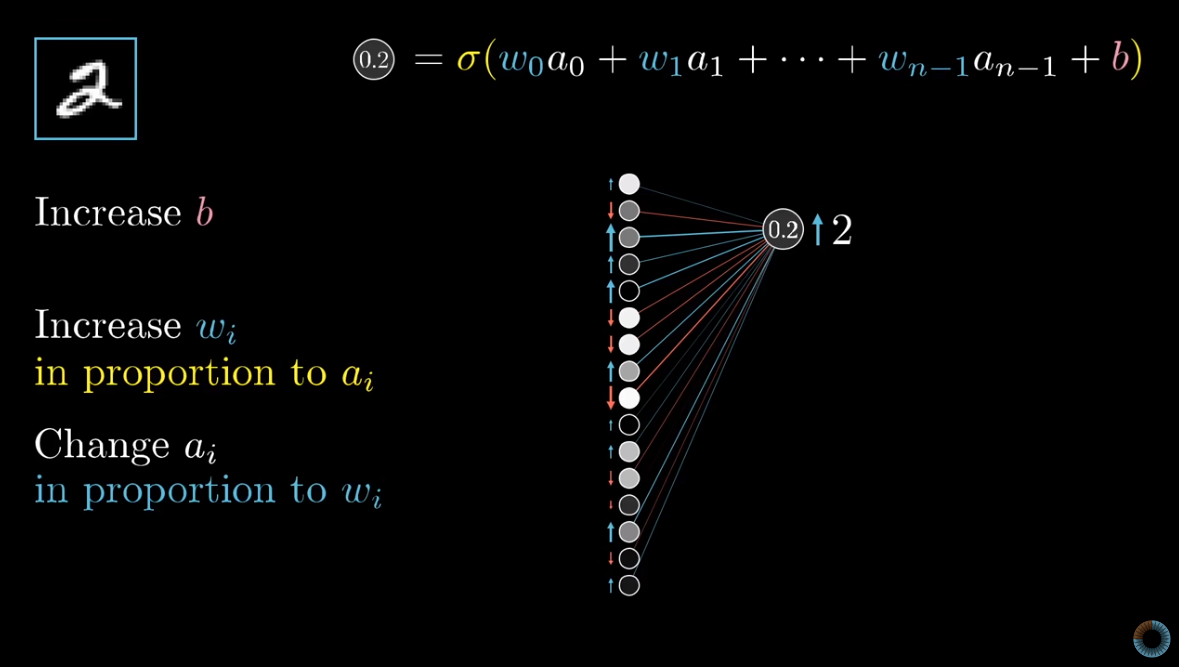
\includegraphics[max width=.9\textwidth]{ai_20}
	\caption{Which weights need to change}
	\label{ai_20}
\end{figure}

To see which parameters need change in detail we first have to take a look at one specific neuron. In this example the one holding the value of two. The \textit{activation} of the neuron depends on multiple factors. To increase the value of the output neuron we can increase the \textit{bias}, increase the weights and we can change the activation from the previous layer.

Importance here: The neuron with a higher weight have a larger influence on the perceiving layer than the ones with a lower one. So its generally a good idea to to increase the weight of lit neurons who already have a larger weight than those who have not. But it's not enough to just look at the weights applied on this particular neuron. It is important to also check with the computed gradient from the cost function to see which of those neurons has the biggest influence on the cost function itself (in the video repeadedtly referred to as \textit{getting the most bang for your bug.}) 

Conclusion: \textit{Those neurons that fire together wire together.} it is important to see that the biggest increase of the weights / the biggest strengthening of connections happens between neurons happens between neurons which are the most active and the ones we \textbf{wish} to become more active. While changing the weights and bias for one specific neuron does not bring change to any of the other neurons on the layer we have to also take in account what the neuron wants. Accourding to this priciple the two \textit{wants} the less active neurons with a negative weight should become more dimmer and the ones with a higher weight and activation should become brighter to overall increase the activation of the neuron itself. 

\begin{figure}[!htbp]
	\centering
	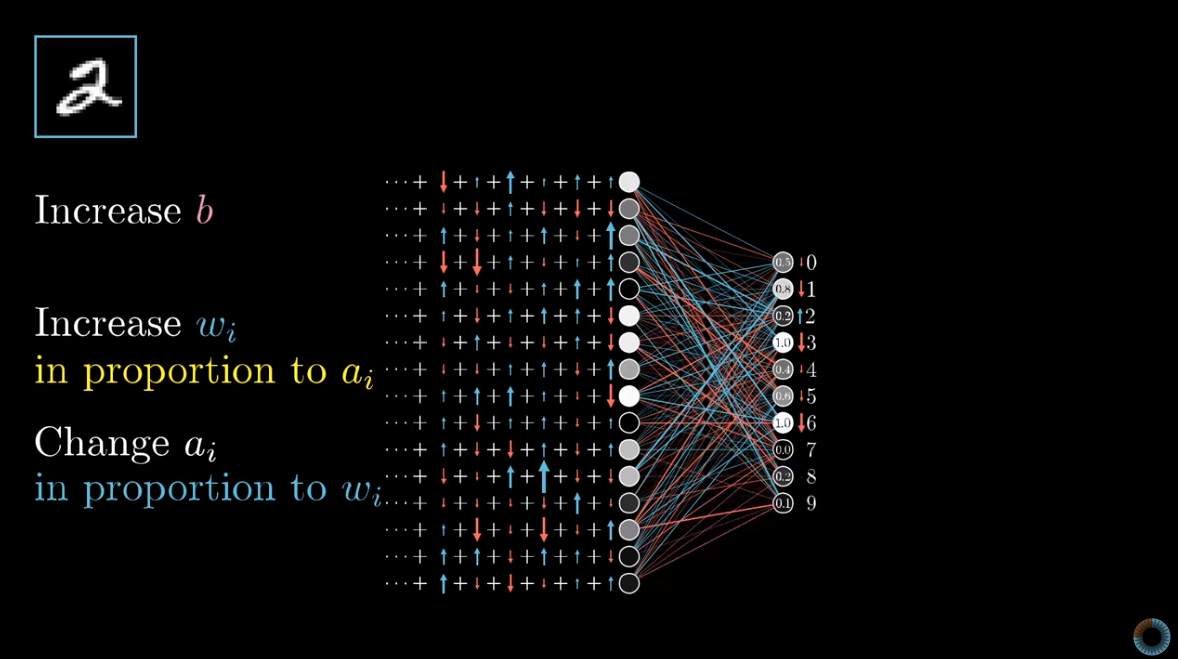
\includegraphics[max width=.9\textwidth]{ai_21}
	\caption{Desired changes - single neuron}
	\label{ai_21}
\end{figure}

But since it is not possible to directly influence the activation of the previous neurons from the last layer, we have to keep track of those \textbf{\textit{wishes}}. Since all the neurons on the same layer apply this principle and can propose their \textbf{wishes} regarding the brightness / activation of the previous layers we can tracked. Afterwards we need to add those desired changes together under the premise of the \textbf{influence} each neuron needs to have accourding to their difference to the optimal solution (discussed on the last paragraph). 

\begin{figure}[H]
	\centering
	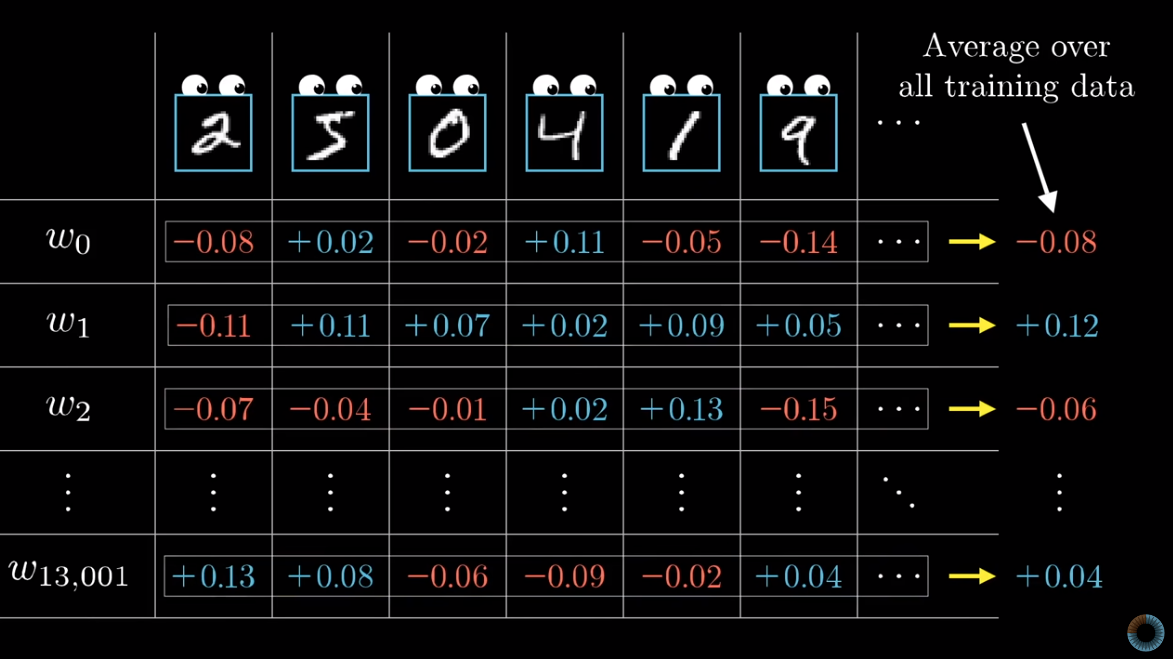
\includegraphics[max width=.9\textwidth]{ai_22}
	\caption{Computing negative gradient vector - Average}
	\label{ai_22}
\end{figure}


% -------------------------------------------------- 

\subsection{Stachastic gradient descent}

After taking in all the desired changes from the top layer we need to apply the same principle to the underlying layer hence \textbf{propagating backwards}. This process describes what needs to happen on for a single test sample. But to lower the cost function for the all samples we need to compute the average for all training data samples. When putting all those together again as an output vector we roughly get the previously mentioned \textit{gradient vector}.

\begin{figure}[!htbp]
	\centering
	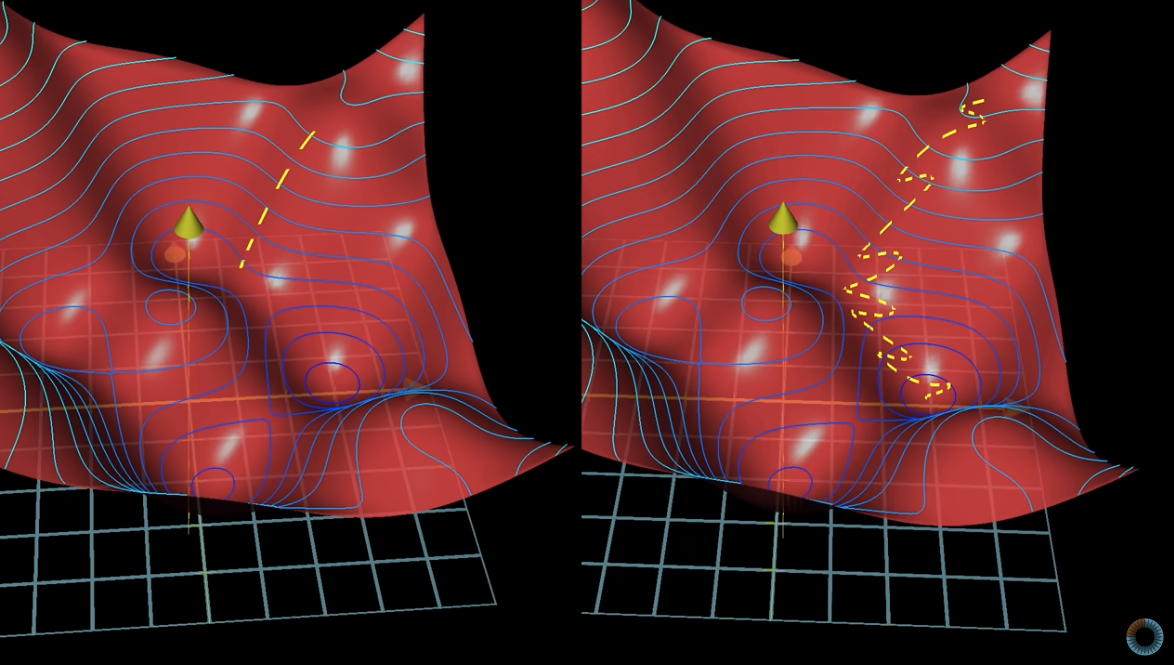
\includegraphics[max width=.9\textwidth]{ai_23}
	\caption{Plotted stochastic gradient descent on 3d space}
	\label{ai_23}
\end{figure}

The only problem with this is that to compute a complete gradient descent step for all samples. In reality the whole collectio of testdata will be subdivided into subsets \textit{(Mini-batches)} with which the steps are not as precise as with the whole set of samples but it is much faster to compute and is also capable of finding the minimum (it only takes more steps). Figure \ref{ai_23} displays what those steps might look like if they were plotted in the simplyfied three dimensional space.





\end{document}
